% F1: GAT-CTDE encoder + per-slice Q-heads (left) and the federated
% training loop (right). Standalone-compilable for iteration; \input{}
% into the paper body. Mirrors paper_conf/figures/fig1_architecture.tex's
% style conventions (box/arrow styles, font, palette).
\documentclass[tikz,border=2pt]{standalone}
\usepackage{amsmath}
\usetikzlibrary{arrows.meta,positioning,fit,backgrounds}

\begin{document}
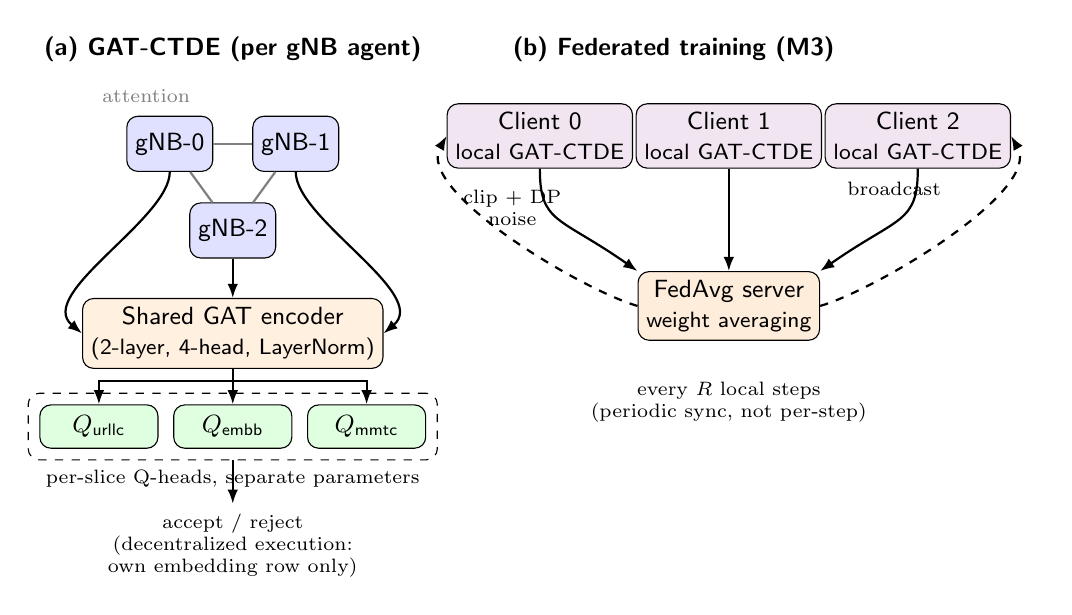
\begin{tikzpicture}[
  font=\sffamily\small,
  box/.style={draw, rounded corners, minimum height=0.7cm, align=center, inner sep=3pt},
  node1/.style={box, fill=blue!12, minimum width=1.0cm},
  node2/.style={box, fill=blue!12, minimum width=1.0cm},
  node3/.style={box, fill=blue!12, minimum width=1.0cm},
  encoder/.style={box, fill=orange!12, minimum width=2.6cm},
  qhead/.style={box, fill=green!12, minimum width=1.5cm, minimum height=0.55cm},
  client/.style={box, fill=violet!10, minimum width=1.8cm},
  server/.style={box, fill=orange!14, minimum width=2.0cm},
  arrow/.style={-{Latex[length=1.8mm]}, thick},
  dashedarrow/.style={-{Latex[length=1.8mm]}, thick, dashed},
]

% ===== Left half: GAT-CTDE per-agent pipeline =====
\node[font=\sffamily\bfseries\small] (lefttitle) at (0,3.3) {(a) GAT-CTDE (per gNB agent)};

% 3-gNB fully-connected graph
\node[node1] (n1) at (-0.8,2.1) {gNB-0};
\node[node2] (n2) at (0.8,2.1) {gNB-1};
\node[node3] (n3) at (0,1.0) {gNB-2};
\draw[thick, gray] (n1) -- (n2);
\draw[thick, gray] (n1) -- (n3);
\draw[thick, gray] (n2) -- (n3);
\node[font=\scriptsize, gray, above=0.05cm of n1, xshift=-0.3cm] {attention};

\node[encoder, below=0.5cm of n3] (gat) {Shared GAT encoder\\\footnotesize (2-layer, 4-head, LayerNorm)};
\draw[arrow] (n1.south) .. controls +(0,-0.6) and +(-0.6,0.5) .. (gat.west);
\draw[arrow] (n2.south) .. controls +(0,-0.6) and +(0.6,0.5) .. (gat.east);
\draw[arrow] (n3.south) -- (gat.north);

\node[qhead, below=0.45cm of gat, xshift=-1.7cm] (q1) {$Q_{\text{urllc}}$};
\node[qhead, below=0.45cm of gat] (q2) {$Q_{\text{embb}}$};
\node[qhead, below=0.45cm of gat, xshift=1.7cm] (q3) {$Q_{\text{mmtc}}$};
\draw[arrow] (gat.south) -- ++(0,-0.15) -| (q1.north);
\draw[arrow] (gat.south) -- (q2.north);
\draw[arrow] (gat.south) -- ++(0,-0.15) -| (q3.north);
\node[draw, dashed, rounded corners, fit=(q1)(q2)(q3), inner sep=4pt,
      label={[font=\scriptsize]below:per-slice Q-heads, separate parameters}] (qbox) {};

\node[below=0.55cm of qbox, font=\scriptsize, align=center] (action) {accept / reject\\(decentralized execution:\\own embedding row only)};
\draw[arrow] (qbox.south) -- (action.north);

% ===== Right half: federated training loop =====
\node[font=\sffamily\bfseries\small] (righttitle) at (5.6,3.3) {(b) Federated training (M3)};

\node[client, minimum width=2.1cm] (c1) at (3.9,2.2) {Client 0\\\footnotesize local GAT-CTDE};
\node[client, minimum width=2.1cm] (c2) at (6.3,2.2) {Client 1\\\footnotesize local GAT-CTDE};
\node[client, minimum width=2.1cm] (c3) at (8.7,2.2) {Client 2\\\footnotesize local GAT-CTDE};

\node[server, below=1.3cm of c2] (server) {FedAvg server\\\footnotesize weight averaging};

\draw[arrow] (c1.south) .. controls +(0,-0.7) and +(-1.0,0.7) .. (server.north west);
\draw[arrow] (c2.south) -- (server.north);
\draw[arrow] (c3.south) .. controls +(0,-0.7) and +(1.0,0.7) .. (server.north east);
\node[font=\scriptsize, align=center, below=0.15cm of c1, xshift=-0.35cm] {clip + DP\\noise};

\draw[dashedarrow] (server.west) .. controls +(-0.7,0.2) and +(-0.4,-0.7) .. (c1.west);
\draw[dashedarrow] (server.east) .. controls +(0.7,0.2) and +(0.4,-0.7) .. (c3.east);
\node[font=\scriptsize, below=0.05cm of c3, xshift=-0.3cm] {broadcast};

\node[below=0.4cm of server, font=\scriptsize, align=center] {every $R$ local steps\\(periodic sync, not per-step)};

\end{tikzpicture}
\end{document}
